\tikzset{every picture/.style={line width=0.75pt}} %set default line width to 0.75pt        

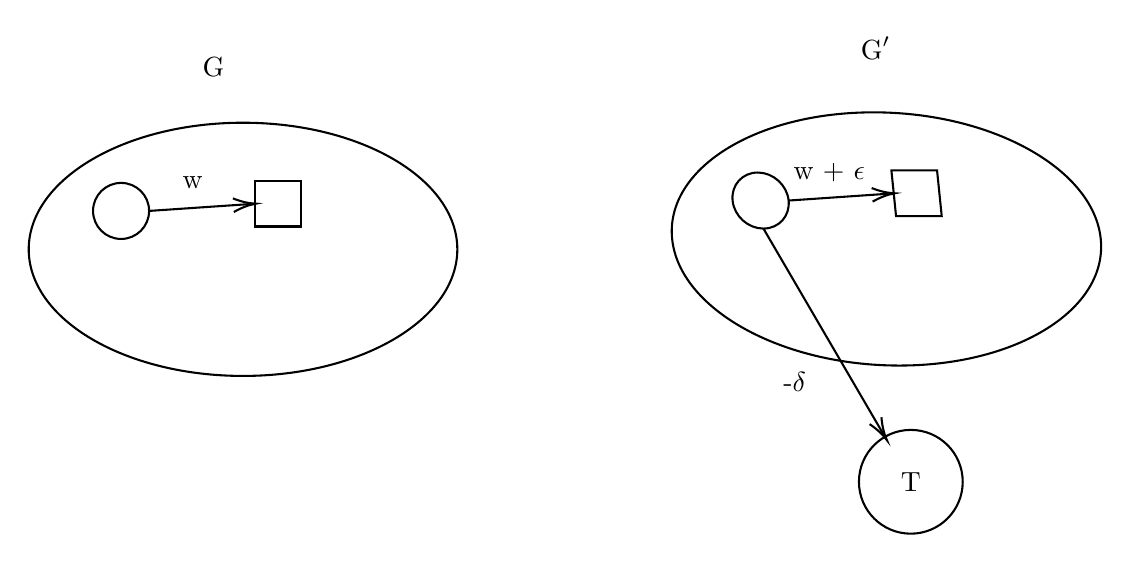
\begin{tikzpicture}[x=0.75pt,y=0.75pt,yscale=-1,xscale=1]
%uncomment if require: \path (0,300); %set diagram left start at 0, and has height of 300

%Shape: Ellipse [id:dp35665433870720253] 
\draw   (28,115) .. controls (28,81.31) and (74.23,54) .. (131.25,54) .. controls (188.27,54) and (234.5,81.31) .. (234.5,115) .. controls (234.5,148.69) and (188.27,176) .. (131.25,176) .. controls (74.23,176) and (28,148.69) .. (28,115) -- cycle ;
%Shape: Circle [id:dp8502084996926933] 
\draw   (59,96.5) .. controls (59,89.04) and (65.04,83) .. (72.5,83) .. controls (79.96,83) and (86,89.04) .. (86,96.5) .. controls (86,103.96) and (79.96,110) .. (72.5,110) .. controls (65.04,110) and (59,103.96) .. (59,96.5) -- cycle ;
%Shape: Square [id:dp9450962306071624] 
\draw   (137,82) -- (159,82) -- (159,104) -- (137,104) -- cycle ;
%Straight Lines [id:da2842158542061044] 
\draw    (86,96.5) -- (135.5,93.14) ;
\draw [shift={(137.5,93)}, rotate = 536.11] [color={rgb, 255:red, 0; green, 0; blue, 0 }  ][line width=0.75]    (10.93,-3.29) .. controls (6.95,-1.4) and (3.31,-0.3) .. (0,0) .. controls (3.31,0.3) and (6.95,1.4) .. (10.93,3.29)   ;

%Shape: Ellipse [id:dp9633483807744296] 
\draw   (338,110) .. controls (334.57,76.31) and (378.02,49) .. (435.04,49) .. controls (492.07,49) and (541.08,76.31) .. (544.5,110) .. controls (547.93,143.69) and (504.48,171) .. (447.46,171) .. controls (390.43,171) and (341.42,143.69) .. (338,110) -- cycle ;
%Shape: Circle [id:dp3748033424118844] 
\draw   (367.12,91.5) .. controls (366.36,84.04) and (371.79,78) .. (379.24,78) .. controls (386.7,78) and (393.36,84.04) .. (394.12,91.5) .. controls (394.88,98.96) and (389.45,105) .. (381.99,105) .. controls (374.53,105) and (367.87,98.96) .. (367.12,91.5) -- cycle ;
%Shape: Square [id:dp9047184358152496] 
\draw   (443.64,77) -- (465.64,77) -- (467.88,99) -- (445.88,99) -- cycle ;
%Straight Lines [id:da04429014923239061] 
\draw    (394.12,91.5) -- (443.26,88.14) ;
\draw [shift={(445.26,88)}, rotate = 536.0899999999999] [color={rgb, 255:red, 0; green, 0; blue, 0 }  ][line width=0.75]    (10.93,-3.29) .. controls (6.95,-1.4) and (3.31,-0.3) .. (0,0) .. controls (3.31,0.3) and (6.95,1.4) .. (10.93,3.29)   ;
\draw   (428,227) .. controls (428,213.19) and (439.19,202) .. (453,202) .. controls (466.81,202) and (478,213.19) .. (478,227) .. controls (478,240.81) and (466.81,252) .. (453,252) .. controls (439.19,252) and (428,240.81) .. (428,227) -- cycle ;
%Straight Lines [id:da29377848783032556] 
\draw    (381.99,105) -- (440.49,205.27) ;
\draw [shift={(441.5,207)}, rotate = 239.74] [color={rgb, 255:red, 0; green, 0; blue, 0 }  ][line width=0.75]    (10.93,-3.29) .. controls (6.95,-1.4) and (3.31,-0.3) .. (0,0) .. controls (3.31,0.3) and (6.95,1.4) .. (10.93,3.29)   ;
\draw (107,83) node  [align=left] {w};
% Text Node
\draw (413.74,78) node  [align=left] {w + $\displaystyle \epsilon $};
% Text Node
\draw (453,227) node  [align=left] {T};
% Text Node
\draw (397,179) node  [align=left] {\mbox{-}$\displaystyle \delta $};
% Text Node
\draw (117,27) node [xslant=0.06] [align=left] {G};
% Text Node
\draw (436,18) node  [align=left] {G$\displaystyle ^{\prime }$};


\end{tikzpicture}